\chapter{Machine learning for quality control} \label{Machine Learning for Quality Control}
\minitoc

\section{Introduction}

In this chapter, we describe a general framework to model the relationship between machine process data and product quality. The method described relies on four consecutive stages: data acquisition, data processing, exploratory data analysis and supervised machine learning modelling. The objectives for the manufacturing company applying this method can be twofold: on the one hand, to determine the process parameters that have a significant influence on the quality of the finished parts. It is then possible to monitor them to ensure their stability over time. On the other hand, the trained model can be used to infer part quality from the process parameters. In this way, it is possible to provide a quality status to each part produced. This is particularly interesting when quality control cannot inspect all the parts produced, which is the case in most companies. By providing the quality status for all parts produced, it is possible to react faster to quality non-conformities and to avoid sending to the customer a part which is non compliant with the specifications.  In the second part of this chapter, the definition of the core concepts and approaches used in machine learning are presented, thus serving as an introduction to the machine learning algorithms and techniques used in this thesis.

\section{Towards data-driven quality control}

In the manufacturing industry, product quality is an indicator of the production capacity of a company. Customers are increasingly demanding in terms of product quality, and providing them with a product that complies with the specifications is absolutely essential in an increasingly competitive market. The ideal solution would be to inspect in details all parts produced, but most companies cannot test every product. This may be due to the production rate being too high to allow inspection at a reasonable cost or within a reasonable time. Quality testing may also result in the destruction of the product or render it unfit for sale in some way. In our industrial context, quality control is a time-consuming operation that requires several minutes of work and that cannot be done online for each part. Only a subset of the produced parts can be inspected. One set of statistical tools for applying such a screening is acceptance sampling. Using such tools enables decision makers to determine what action to take on a batch of products. Decisions based on frequency testing, rather than on a thorough inspection, are more expedient and cost effective but they cannot guarantee the conformity of all parts of the population from which the sample was drawn~\citep{fuchs1998multivariate}. Figure \ref{fig:statistical_quality_control} describes acceptance sampling. 

\begin{figure}
\centering
\includegraphics[scale=0.50]{images/chapter_4/statistical_quality_control.png}
\caption{Statistical quality control}
\label{fig:statistical_quality_control}
\end{figure}

Although this method is widely applied and accepted in the manufacturing industry, it presents three major drawbacks:
\begin{enumerate}
    \item Acceptance sampling is able to track deviations in product quality, but it  may happen that one or more non-compliant parts produced during a temporary malfunction are not detected. These non-compliant parts are then sent to the customer.
    \item Acceptance sampling incurs delay in detecting process deviations. If the quality of the product starts to deviate, the manufacturer does not identify the problem until the next quality control, so the process is not corrected immediately. The parts produced in this time frame are potentially non-compliant and require extra time-consuming quality control to establish whether or not the parts can be sent to the customer.
    \item Some quality controls require the destruction of the part or a modification that makes it unsuitable for sale. For instance, advanced quality control for assessing the material distribution of each thickness layer of a blow-moulded part requires the part to be cut into small samples, which are then analysed in the laboratory. Even if these tests are necessary to certify the part conformity, they increase the number of PPM (parts per million) waste.
\end{enumerate}

In order to improve quality control, we seek to achieve a comprehensive quality control using a machine learning based approach, where the quality status of each part produced is inferred by a data-driven model. 
This ensures a control of all parts produced, which enables for a fast reaction to quality non-conformities (Figure \ref{fig:model_quality_control} on the left side). In fact, by ``virtually'' measuring each part, we may eventually discard parts for which the model has provided a ``Not-OK'' result, or request the quality team to carry out more in-depth tests. Model-based quality measurement may be effectively used to detect those parts that turn out to be, from a statistical point of view, outliers. In this way, instead of randomly sampling the parts to be measured by the quality operators, the model may suggest parts that seem to be interesting.
If the trained model is sufficiently accurate and robust, the real quality controls which destroy the parts or make them unusable could be reduced (Figure \ref{fig:model_quality_control} on the right side). In such a case, not only the model-based control would be able to provide a thorough quality control, but it would also be able to reduce the scraps which account for an overall better production performance. Of course, real measurements cannot be completely replaced by model-based measurements: real measurements are the primary data sources to train and to validate the data-driven model. 

\begin{landscape}
\begin{figure}
\centering
\includegraphics[scale=0.50]{images/chapter_4/data_driven_model.png}
\caption{Data-driven model-based quality control}
\label{fig:model_quality_control}
\end{figure}
\end{landscape}



\section{General method} \label{Proposed Method}

In this section, we describe a general framework for dealing with predictive quality topics. We use supervised machine learning to discover patterns between process parameters and the quality of the parts that have been manufactured by that process. We proceed in four main stages:
\begin{enumerate}
    \item \textit{Data collection} consists in retrieving all the data needed to train the machine learning model It involves two main stages:  data acquisition and  data labelling (see Section \ref{Data Collection}). 
    \item \textit{Data processing} covers the operations required to make the data suitable for the machine learning algorithm (see Section \ref{Data Processing}). 
    \item \textit{Exploratory data analysis} is an ensemble of graphical and quantitative techniques that can be used to explore data and retrieve important information (see Section \ref{Exploratory Data Analysis}).
    \item \textit{Data modelling} corresponds to the statistical modelling of the relationship between the process data and the quality data by the machine learning algorithm (see Section \ref{Machine Learning modeling})
\end{enumerate}
The remaining part of the current section describes these four stages. 

\subsection{Data collection} \label{Data Collection}

In order to train a machine learning model, it is necessary to have samples that are representative of the entire operating range of the process. Iconic applications of machine learning, such as machine translation or object detection in images, rely on huge amounts of training data, but in new applications, such as in manufacturing, the training data is often limited.

Collecting data allows to capture a record of past events so that we can use data analysis to find recurring patterns. In the context of this research work, data collection is the task of retrieving the data that could be meaningful to explain the quality of parts given some process parameters. Among the many challenges in Industry 4.0, data collection is becoming one of the critical bottlenecks. It is known that the majority of the time for building end-to-end data-driven models is spent on preparing data, which includes collecting, cleaning, analysing, visualising, and feature engineering. 

Two kind of data are required: input data, corresponding to the process data and output data which is actually the measurement of the part quality. Data collection involves two different steps: \textit{process data acquisition} and \textit{quality data acquisition}. 

\subsubsection{Process data acquisition} \label{Process Data Acquisition}

We use here the term \textit{process data} for any type of data belonging to the manufacturing process. For instance, for extrusion blow-moulding such data are extruder throughputs, extruder temperatures, or blowing air pressures. This process data pictures the process state at a given time.

Process data acquisition is a challenging task in Industry 4.0 due to different technologies, machines, sensors, IoT devices and communication networks. Sensors, actuators, and Programmable logic controllers (PLCs) are the main data generators in the automotive industry \citep{khan2017big}. In the last decade a new type of intelligent sensor, also called \textit{smart sensors}, is more and more used in the manufacturing industry. Most of the data available in the manufacturing plants comes from PLCs, sensors and smart sensors. The three devices are further explained as below.

\begin{itemize}
    \item \textit{PLC} is a programmable unit that takes input from sensors, and controls actuators (Figure \ref{fig:plc}). A factory has a large number of PLCs which controls the machines. PLCs are manufactured by different suppliers and generate heterogeneous data, which is a big challenge for industrial big data.
    \item \textit{Sensors} convert a physical state or activity into an electrical signal that is sent to the PLC for further processing. In manufacturing, sensors create a huge amount of data. Most machines and robots include sensors that collect data from their surroundings, such as temperatures of machine components or its environment.
    \item \textit{Smart sensors} are devices that take information from a physical environment and use embedded microprocessors and wireless communication to monitor, examine and provide information about the proper functioning of the observed system. With the developments of IoT and machine learning, various types of smart sensors are nowadays available.
    \item \textit{Actuators}, controlled by the PLC, produce a physical action. A basic example of an actuator connected to a PLC is the automatic starting of a motor. 
\end{itemize}
%
\begin{figure}
\centerline{\includegraphics[scale=1]{images/chapter_3/PLC.jpg}}
\caption{Programmable logic controller \textit{Siemens} S7-1500}
\label{fig:plc}
\end{figure}
%
All these devices produce a lot of data but they do not manage data storage. PLCs have a limited amount of storage space and cannot be used to store data permanently. The local machine data storage is most of the time handled by the SCADA (Supervisory Control And Data Acquisition) software. The term SCADA is used to identify any kind of software, installed on a personal computer or server, which allows the implementation, operation and management of supervisory, control and remote control systems without necessarily having to write code using programming languages. SCADA software have multiples functionalities which range from automation to alarm handling, logging, archiving and simple statistical analysis \citep{daneels1999scada}. 
The data collected by the SCADA system is stored in a place where data is easily accessible, such as a cloud platform, whether internal to the manufacturing company or external. Cloud platforms, or \textit{data lakes}, are designed to be highly scalable and provide a way to easily access data through Big data technology that facilitates and accelerates data analysis stages.  

In order to be able to properly manage data acquisition, taking into account the heterogeneity of data coming from the different data sources, we propose to introduce a \textit{gateway} system which constitutes an intermediary bridge between the shop floor PLCs, sensors, and the cloud platform where data is stored. Moreover, it can communicate with the \textit{MES} system. The Manufacturing Execution System (MES) is a production management system serving as the information center in the enterprise to improve manufacturing transparency. It is the middle layer connecting the manufacturing process on the shop floor and the business process on the Enterprise Resource Planning (ERP) \citep{chen2020implementation}. By communicating with the MES system, it is possible to associate to a produced part the set of events that have enabled its production. The architecture of the overall data acquisition system is shown in Figure \ref{fig:data_acquisition_architecture}.

The gateway is a physical or virtualised server which acts as an intermediary between data acquisition systems available in the shop floor and the cloud platform where data is stored for data analysis. The gateway is connected to the shop floor network and it is able to interact directly with machine PLCs as well as smart sensors. The gateway has two main roles:

\begin{itemize}
    \item It allows to centralise the data collection at plant level. It is in charge to retrieve data from all data sources, whether they are PLCs, smart sensors, SCADA software or the MES system. This process facilitates the subsequent sending of data to the cloud platform. 
    \item This gateway is well suited  to the eventual deployment on site of the machine learning models that have been trained. 
\end{itemize}
%
The gateway should be equipped with different tools and software to allow the communication with machines through different communication protocols used in Industry 4.0. There exist a multitude of communication protocols. Among all these we can mention \textit{OPC UA} and \textit{MQTT}. OPC UA (Open Platform Communications Unified Architecture) is a service-oriented machine-to-machine communication protocol mainly used in industrial automation. Its main goals are to provide a cross-platform communication protocol while using an information model to describe data transfer. MQTT (Message Queuing Telemetry Transport) is an open message protocol which mainly focuses on a small code footprint and low network bandwidth usage, while handling high latency or bad network connections \citep{profanter2019opc}. Further information regarding communication protocols used in Industry 4.0 are available in \citet{profanter2019opc}, \citet{8262021} and \citet{zezulka2018communication}.

\begin{landscape}
\begin{figure}
\centering
\includegraphics[scale=0.5]{images/chapter_3/Data_acquisition_architecture.png}
\caption{Data acquisition architecture}
\label{fig:data_acquisition_architecture}
\end{figure}
\end{landscape}

\paragraph{Process data types}

When dealing with process data, we distinguish two different types of data: \textit{cyclical data} and \textit{time series data}.

\begin{itemize}
    \item \textit{Cyclical data} are scalar values which provide information about a certain recurring event. Examples of cyclical data are the machine cycle time, or the time needed by the machine to perform an operation. 
    \item \textit{Time series} are sequential data that aggregate several sequential values of the same process parameters. For instance, the temperature of a machine component may be measured throughout the production cycle. The number of sequential values composing the time series depends on the sampling rate and may change according to the nature of the measurement.
\end{itemize}

\begin{figure}
\centering
\includegraphics[scale=0.5]{images/chapter_3/time_series_data.png}
\caption{Time series}
\label{fig:time_series_data}
\end{figure}


\subsubsection{Quality data acquisition}

Quality data acquisition consist in collecting product quality data associated with all or some of the parts produced. The quality label can be continuous or discrete. For instance, the thickness of a manufactured part can be reported in the form of continuous values in meters, or can be directly associated with a class according to its compliance, or non-compliance, with the specifications. If the label is categorical, the  modelling problem is a classification problem, if the label is continuous,  it is a regression problem (see Section \ref{Classification}). Quality data acquisition can be done offline or online, as detailed in the following paragraphs. 

\paragraph{Offline acquisition}

Offline acquisition, is the most common approach for the quality labelling of manufactured parts. In fact, for all non-visual product characteristics, it is extremely complicated to assess the quality of part in less then a minute. Most of quality controls on parts require specific equipment and the task of controlling can take several minutes. Moreover, effective control might result in the destruction of the product or render it unfit for sale. In such a case, the only option is to measure the part quality offline. Measuring offline has the advantage of allowing careful control of the manufactured parts, reducing the possibility of measurement error. However, as there are only a few parts measured, it may take a long time to build a dataset that is representative of all categories of part non-compliance. As quality is not measured on all parts produced, it is crucial to structure the data collection to facilitate access for future data analysis. In the database, the quality measurement must be related to a part number, or traceability number, in order to then associate it with the process data, which in turn must be tagged with the part number.

\paragraph{Online acquisition}

Performing online data acquisition, on the production line, eliminates two critical error risks:
\begin{enumerate}
    \item The loss of the link between production measurements and off-line annotation.
    \item The transformation of parts between their production and their annotation.
\end{enumerate}
%
On the other hand, the time available for annotation is very limited. Most of the time, machine operators have time constraints to meet the production rate, so that their annotation must be done in a limited amount of time. This time may vary depending on the operator's charge. We estimate that the operator can allocate a maximum of one third of the production cycle time to this task, which means that for a process with a cycle time of 60 seconds the operator has at maximum 20 seconds to perform it. In addition to annotation time, the operator has to assist in the handling of the parts and related operations.

By automating the process data acquisition through the data collection presented above, and by ensuring the proper recording of the quality of parts, it is possible to permanently feed a dataset with new data automatically. Over time, it is hoped that enough data can be recovered to cover the entire distribution of all possible quality non-conformities. 

\subsection{Data processing} \label{Data Processing}

The heterogeneous data collected require processing to make them suitable to data analysis. In general, data processing comprises three major tasks: data cleaning, reduction, and scaling.
In the remaining part of this section we will provide some additional elements regarding these three data processing tasks. 
  
\subsubsection{Data cleaning}

Data cleaning is the result of two main operations: missing values imputations and outlier removals.
For handling  missing data, the first option is simply to reject data samples with missing values to allow the use of the numerous data mining algorithms that cannot handle missing data. This approach is only possible when the amount of missing values is small. The second technique is to impute the missing values, that is, to replace missing values with inferred ones. Mean imputation, forward or backward imputation, or moving average are examples of standard imputation procedures. In these techniques, missing values are inferred based solely on the data properties of that variable, and therefore are referred to as univariate techniques. The mean or median imputation method will replace missing values with the mean or median of that variable. The forward or backward method simply updates the missing value with the previous or next data measurement. More advanced techniques make use of multivariate predictors to obtain more accurate imputation results. 

As regarding outlier removals, the most common techniques use statistical analysis to identify atypical data. Data outliers can be identified, for instance, if the data falls beyond a certain range constructed using conventional statistics such as standard deviations, means and quantiles. Identifying outliers is delicate because what at first sight might appear to be an outlier may turn out to be extremely interesting data. When dealing with manufacturing process data, the outlier can be representative of a process operating condition that is not normal and could therefore explain some product quality non-compliances. Physical knowledge of the production process is therefore indispensable in order to understand whether the outliers are due to a process malfunction or to a data acquisition error.    


\subsubsection{Data reduction}

Data reduction aims to reduce data dimensions. Assuming that data are in a tabular format where the row represents the samples and columns the features, or process parameters, data reduction may be conducted to reduce either the number of rows or the number of columns.
There are three main methods of column-wise data variable reduction: The first is to use domain knowledge to directly select the variables of interest. The second is to use statistical feature selection methods to select important variables. The third is to adopt feature extraction methods to construct useful aggregated features.
Human expertise plays a key role in the data acquisition process and, globally, in tasks of modelling by the relationship between process parameters and product characteristics. For complex processes, the number of available process parameters are huge, in the order of hundreds and sometimes thousands. The knowledge of human experts on the process may allow to pre-select a number of useful features that can be used to try predicting the target output. 

As regarding feature selection techniques, we distinguish mainly three approaches: filter, wrapper and embedded methods. Filter methods are simple approaches where variables are ranked and selected based on specific univariate metrics. Pearson's correlation coefficient is a common filter technique for determining the direction and strength of a linear relationship between two variables. 

Wrapper methods assess the usefulness of data variables for a given learning algorithm. Heuristic search methods, such as stepwise forward and backward selection methods, are commonly used. Compared to the filter approach, the wrapper methods take into consideration data variable correlations and interactions with learning algorithms. However, because it is generally performed via trial and error, the computing costs associated with wrappers is significantly higher. 

Embedded approaches select features during the training of the model. A popular embedded method is L1 regularisation (based on the least absolute shrinkage and selection operator, Lasso).

\paragraph{Stability selection} \label{Stability Selection}

Stability selection \citep{meinshausen2010stability} has been extensively used in this research work. This technique consuists in injecting noise into the original problem by generating bootstrap samples of the data (see Section \ref{Tree-based methods}), and to use a learning algorithm to find out which features are important in every bootstrap sample of the data. For a feature to be considered important, it has to be selected often among the perturbed versions of the original problem. This tends to filter out features that are only weakly related to the target variables, because the additional noise introduced by the bootstrapping breaks that weak relationship. The algorithm takes as input a grid of values $\Lambda$ for the regularisation parameter $\lambda$, and the number of bootstrap samples $B$ to be generated. Stability selection returns a selection probability $\hat{\Pi}^{\lambda}_{k}$ for every value $\lambda \in \Lambda$ and for every feature $k$, and the set of stable features $\hat{S}^{stable}\subseteq\{1,\ldots,p\}$. The algorithm consists of two steps. In the sampling step the selection probabilities, or stability scores, are computed as follows. For each value $\lambda \in \Lambda$ do:

\begin{itemize}
    \item For each $i$ in $1,\dots, B$, do:
    \begin{itemize}
        \item Generate a boostrap sample of the original data (that is, a sample of size $n$ formed by $n$ independent draws with replacement of the original data).
        \item Run the selection algorithm on the boostrap sample with regularisation parameter $\lambda$ to get the selection set $\hat{S}^{\lambda}_{i}$.
    \end{itemize}
    \item Given the selection operated on each boostrap sample, calculate the proportion of models selecting variable $k$:
    \begin{equation*}
        \hat{\Pi}^{\lambda}_{k} = \frac{1}{B}\sum_{i=1}^{B} \mathds{I}_{k \in \hat{S}^{\lambda}_{i}}
        \enspace.
    \end{equation*}
\end{itemize}
%
In the scoring step, the set of stable features is defined as follows:

\begin{equation*}
    \hat{S}^{stable} = \{k:\max\hat{\Pi}^{\lambda}_{k} \geq \pi_{thr}\}
    \enspace,
\end{equation*}
%
where $\pi_{thr}$ is a predefined threshold. When the stability score for a variable exceeds the threshold $\pi_{thr}$ for one value in $\Lambda$, it is deemed stable. In practice the Lasso penalisation (see section \ref{Parametric models}) is frequently applied to get the selection set $\hat{S}^{\lambda}_{i}$. This is due to the ability of Lasso to perform exact selection.

Unlike feature selection, which picks relevant features from existing variables, feature extraction seeks to create new aggregated features, built by linear or nonlinear combinations of existing variables. Principal Component Analysis (PCA) is such a common linear feature extraction technique. The principal components are linear combinations of the original data variables that can be used as new features. PCA is particularly useful when there are collinearity problems. In practice, the number of principal components, or features extracted, is determined based on the proportion of total data variance explained; for instance, the principal components may explain at least 80 or 90\% of the total data variance. More advanced techniques, such as \textit{auto-encoders} \citep{rumelhart1985learning}  extract nonlinear features. When dealing with time-series data we can compress the entire information in a limited set of new features computed through the use of summarising statistics, such as the mean, peak, and standard deviation over a particular time span.

\subsubsection{Data scaling} \label{Data Scaling}

Data scaling aims to transform the original data into homogeneous ranges. It is necessary if the results are not to depend on the units of measurement chosen. The most used scaling techniques are \textit{max-min normalisation} and \textit{z-score standardisation}. Min-max normalisation is defined as follows: 
\begin{equation*}
    x = \frac{x - x_{min}}{x_{max} - x_{min}}
    \enspace,
\end{equation*}
%
where $x_{min}$ and $x_{max}$ refer to the minimum and maximum values of the generic feature $x$. The z-score standardisation is instead defined by the following equation:

\begin{equation*}
    x = \frac{x - \mu}{\sigma}
    \enspace,
\end{equation*}
%
where $\mu$ is the mean and $\sigma$ is the standard deviation of the feature $x$.

Z-score standardisation is well suited when data are normally distributed.
The max-min normalisation, instead, is recommended when the data do not conform to a normal distribution and have no outliers. 

\subsection{Exploratory data analysis} \label{Exploratory Data Analysis}

Exploratory Data Analysis (EDA) is a set of data analysis techniques that may be applied to:
%
\begin{itemize}
    \item uncover underlying structures,
    \item isolate important variables,
    \item detect outliers and other anomalies,
    \item suggest suitable models for conventional statistics.
\end{itemize}
%
EDA is usually the intermediate stage between data processing and machine learning modelling. By exploring the data, it is possible to discover interesting patterns among data and drive the modelling phase depending on what have been observed. Moreover, EDA allows to fine-tune the data processing stage. In fact, by exploring the data we can identify useless features that cannot bring any added value and can therefore be discarded.   
The term “Exploratory Data Analysis” was introduced by \citet{tukey1977exploratory} shows how simple graphical and quantitative techniques can be used to explore data.

Typical graphical techniques are:

\begin{itemize}
    \item plotting the raw data (i.e. histograms, scatter plots),
    \item plotting simple statistics (i.e. box plots, residual plots),
\end{itemize}

Typical quantitative techniques are:

\begin{itemize}
    \item interval estimation,
    \item measures of location or of scale,
    \item shapes of distributions.
\end{itemize}
%
A very convenient exploratory data analysis tool is principal component analysis (see Section \ref{Principal Component Analysis}). By projecting input data onto the first principal components, which capture the most variability in the data, it is possible to visualise some interesting global patterns within data, even if the number of features is large. 

\subsection{Supervised learning modelling} \label{Machine Learning modeling}

The objective of a machine learning algorithm is to \textit{generalise from examples}. In supervised learning, this goal is formalised as finding a function $g(\cdot)$ that maps the features to the response variable. 
Generalising from examples means then to \textit{accurately predict the value of the response from the function $g(\cdot)$ on future examples, based on a finite set of examples}, the training set. 
To formalise what future examples look like, it is assumed that they will be drawn from a distribution, and it is assumed that the training set has also been drawn from this distribution, so that it provides relevant clues for the learning objective.
We therefore assume the existence of random variables for the features and the response; these random variables will be respectively denoted by $X$ and $Y$. The (in)accuracy of predictions will be measured by a loss function $L(Y,g(X))$, also called cost function, which represents the loss incurred by predicting $g(X)$ instead of $Y$. The generalisation goal is then to minimise the so-called \textit{risk}:

\begin{equation}\label{eq:risk}
    R(g) = \mathbb{E}_{XY}[ L(Y,g(X))]
    \enspace .
\end{equation}
In practice, this objective cannot be achieved because the distribution of $(X,Y)$ is not known, so the risk $R(g)$ cannot be computed.
With the training set, it is however possible to compute a Monte-Carlo approximation of the risk, called the \textit{empirical risk}, which is the average loss function on the training set:

\begin{equation*}
    R_\mathrm{emp}(g) = \frac{1}{n}\sum_{i=1}^{n}L(y_i,g(x_i)) \enspace,
\end{equation*}
where $n$ is the number of training examples $(x_i,y_i)$. 
Learning then consists in minimising $R_\mathrm{emp}(g)$. 
This minimisation is performed on a fixed class of functions $\mathcal{G}$, for reasons that will not be explained here, but the theory states that this restriction is necessary \citep{vapnik2000nature}. To convince oneself, it is sufficient to consider that all the functions that interpolate the training set are not necessarily interesting in terms of generalisation, since their behaviour between examples can be very different. Moreover, if the responses $y_i$ are noisy, the function $g(\cdot)$ that minimises the risk \eqref{eq:risk} does not necessarily interpolate the training examples.

The training phase, also called the learning phase consists in the minimisation over $\mathcal{G}$ of the average loss computed on the training set:

\begin{equation}\label{eq:riskemp}
    \hat{g} = \argmin_{g\in\mathcal{G}}  R_\mathrm{emp}(g)
    \enspace
\end{equation}
and the function $\hat{g}$ is thus the output of the learning algorithm. 
In practical applications, the available data is usually split in two parts: a training set and a test set. The training is used to estimate the function $\hat{g}$ by solving \eqref{eq:riskemp}, and the test set is used to evaluate the risk $R(\hat{g})$ \eqref{eq:risk} unbiasedly. 
Indeed, for any function chosen independently from the training set, $R_\mathrm{emp}(g)$ is an unbiased estimate of $R(g)$, but this is not true for $\hat{g}$, which minimises $R_\mathrm{emp}(g)$: it is easy to show that $R_\mathrm{emp}(\hat{g})$ is an optimist estimate of $R(\hat{g})$. 

In the context of our research work, supervised learning modelling consists of using of machine learning algorithms to estimate the transfer function between input process data $X=(X_1,X_2,\ldots,X_p)$ and output quality data $Y$ from experimental data. In the following section, we will provide more insights about the machine learning algorithms that we have applied throughout our research work.

\section{Machine learning and deep learning} \label{Machine learning and Deep Learning}

Machine learning (ML) is a field of computer science that aims to give computers the ability to learn and decide without being explicitly programmed. Instead of explicitly encoding knowledge by machine instructions, machine learning leverages data analysis, which involves building and fitting models, to allow machines to ``learn'' from experience. Over the years, a myriad of different kinds of machine learning algorithms and models have been devised for serving different situations and types of problems. 

In everyday life, machine learning is often mistakenly confused as Artificial Intelligence (AI). Figure \ref{fig:ai_ml_dl} locates  machine learning, deep learning and artificial intelligence in relation to each other.
%
\begin{figure}
\centerline{\includegraphics[scale=0.8]{images/chapter_2/AI_ML_DL.png}}
\caption{AI-Machine learning-Deep learning}
\label{fig:ai_ml_dl}
\end{figure}
%
Artificial intelligence is a technology which enables a machine to simulate human behaviour. AI may use, among other ones, one or several machine learning algorithms to learn from past data to solve complex tasks. Deep learning (DL) is a sub-field of ML focusing on deep neural network architectures. Deep-Learning models provide the top performances in numerous applications and challenges. Great improvements have been reached in multiple domains: from web search to image recognition and classification through convolutional neural networks to natural language preprocessing with Recurrent neural networks and \textit{self-attention} networks \citep{vaswani2017attention}. The democratisation of the different models through open-source software libraries, specialised chip-set and highly scalable computing platforms has pushed companies to integrate these tools within their own production facilities. 

In what follows, we review some concepts of machine learning in order to provide the reader with the elements to understand the following chapters. First, the key concepts, such as \textit{supervised} and \textit{unsupervised} learning are presented. Then, we describe the algorithms that have been applied throughout the study. This review is by no means exhaustive but aims to provide the elements necessary for understanding the approaches presented in Chapters \ref{From Corrective to Predictive Process Control} and \ref{Thickness inference using thermal imaging}. Exhaustive reviews of machine learning can be found in \citet{bishop2006pattern,friedman2017elements}. An exhaustive overview of DL architectures is beyond the scope of this research work: research in deep learning is advancing very fast and new architectures are being proposed every day. The end of this section will however describe three types of neural networks: feed-forward neural network, convolutional neural network and recurrent neural network, as well as some specific architectures that we will extensively use in Chapter \ref{Thickness inference using thermal imaging}. For further reading on this topic, \citet{goodfellow2016deep} provides a comprehensive review of the main principles of deep learning. 


\subsection{Supervised learning}

Supervised learning, the most widely used machine learning approach, aims at learning a function from examples of inputs and outputs pairs. The main objective is to accurately predict the responses for future observations (prediction), and a side goal may be to better understand the relationship between the response and the inputs. In general, supervised learning problems are formalised as optimisation problems, by looking for a function that minimises an error criterion that quantifies the discrepancy between predictions and the real value (or “ground-truth”) associated. The cost function should be defined to reflect the cost associated with errors and should be optimisable. We will present below the most common costs in regression and classification.

\paragraph{Regression} \label{Regression}

Regression corresponds to a training objective where training data and their corresponding outcome, a set of numerical continuous variables, are known and available for training. For instance, in a manufacturing context, a regression model can be designed to predict the numerical value of some dimensional characteristic of a manufactured part, given a set of input process parameters. The loss functions used to train regression models are most often based on average distances. The most common and convenient loss function used for regression problems is squared error loss $L(Y, g(X))=(Y-g(X))^2$, leading to:

\begin{equation*}
    R_\mathrm{emp}(g) = \frac{1}{n}\sum_{i=1}^{n}(y_i - g(x_i))^2
    \enspace.
\end{equation*}
where we recall that $(x_i,y_i)$ are the input-output pairs from the training sample of size $n$. 


\paragraph{Classification} \label{Classification}

When the objective is to predict a categorical variable, or class, supervised learning takes the name of classification. In a manufacturing context, a classifier can be trained to recognise whether a part is compliant (OK), or not (NOK), to some quality specification. In classification problems we aim to reduce the misclassification error. In practice, this leads to a combinatorial problem that is hard to solve. For this reason, we generally estimate the probability that a certain sample belongs to a specific class $c$. In this context, the function $g$ maps the features to the $c$ class probabilities, and $g_j(x_i)$ refers to the estimate of the posterior probability $P(Y=j|X=x_j)$. The standard loss function in this case is the cross-entropy, which is also the neg-log-likelihood: 
\begin{equation*}
    L(y_i, g(x_i)) = - \sum_{j=1}^c y_{ij}\log(g_j(x_i))
    \enspace,
\end{equation*}
where $c$ is the number of classes, $y_i$ is the indicator vector of class labels for features $x_i$, that is, $y_{ij}=1$ if $x_i$ belongs to class $j$ and $y_{ij}=0$ otherwise (all examples belong to a single class).

In \textit{binary classification}, where there are only two classes, $y_i$ can be encoded as a simple binary variable, and the loss function becomes:
\begin{equation*}
    L(y_i, g(x_i)) = - y_i \log(g(x_i)) + (1-y_i) \log(1-g(x_i))
    \enspace.
\end{equation*}

\paragraph{Model evaluation}

For the evaluation and comparison of model performances, different performance metrics can be applied. For binary classification, several metrics can be calculated based on the entries of the confusion matrix shown in Table \ref{tab:confusion_matrix}.
%
\begin{table}
\caption{Entries of a confusion matrix}
\label{tab:confusion_matrix}
\begin{tabular}{l|l|l|}
\multicolumn{1}{l}{} & \multicolumn{1}{l}{Actually Positive}              & \multicolumn{1}{l}{Actually Negative}             \\ 
\cline{2-3}
\multicolumn{1}{l|}{Predicted Positive} & \textbf{True Positives (TPs)}  & \textbf{False Positives (FPs)} \\ 
\cline{2-3}
\multicolumn{1}{l|}{Predicted Negative} & \textbf{False Negatives (FNs)} & \textbf{True Negatives (TNs)}  \\ 
\cline{2-3}
\end{tabular}
\end{table}
%
The comparison of the predicted class with the true class allows to distinguish between positive or negative examples correctly classified (true positive, true negative) and incorrectly classified examples (false positive, false negative). This is suitable to discriminate between conforming parts (OK) and non-conforming parts (NOK). 

For regression, the most common metrics to compare model performance are mean squared error (MSE), the root mean squared error (RMSE) and the $R^2$. MSE corresponds to the average of the squared error loss. The root mean squared error (RMSE) is the square root of the MSE: $\mathrm{RMSE} = \sqrt{\mathrm{MSE}}$. RMSE has the advantage of being in the unit of measurement of the target variable. This provides a more direct interpretability of the final result.
The coefficient of determination $\mathrm{R}^\mathrm{2}$ is the proportion of the variance in the dependent variable that is predictable from independent variables:
\begin{equation*}
    \mathrm{R}^2 = 1 - \frac{\mathrm{RSS}}{\mathrm{TSS}} = 1 - \frac{\sum_{i=1}^{n} (y_{i} - g(x_i))^{2} }{\sum_{i=1}^{n} (y_{i} - \bar{y}_{i})^{2}}
    \enspace,
\end{equation*}
where $\mathrm{RSS}$ is the residual sum of squares, $\mathrm{TSS}$ is the total sum of squares and $\bar{y}_{i}$ is the average value of $y_{i}$, $\bar{y}_{i} = \frac{1}{n} \sum_{i=1}^{n} y_{i}$. Values of the coefficient of determination range, normally, from zero (poor model) to one (perfect model), but can be negative when the model does not follow the trend of the data, leading to a worse fit than the average value of the target variable.
As the a-priori selection of adequate algorithms is generally not feasible \citep{kotthoff2016algorithm}, different models need to be evaluated and compared for each industrial application \citep{lee2020machine}. A pre-selection can be made on the basis of criteria such as complexity, interpretability, and speed. 
From a practical point of view, the scoring time of the model should be short enough to adjust the production process in real-time. The required response time depends on the manufacturing process. The scoring time is affected not just by the algorithm employed, but also by the hardware and software on which it is implemented. However, in most situations, the scoring time does not constrain the model selection process.


\subsubsection{Linear models} \label{Parametric models}

Linear models are of the form:
\begin{equation} \label{eq:linear_function}
    g(X) = \beta_1X_1 + \beta_2X_2 + \ldots + \beta_pX_p
    \enspace,
\end{equation}
where $\beta_j$ is the generic $j$-th coefficient, associated with the $j$-th feature.\footnote{%
This expression allows for an intercept if a constant feature $X_0$ is added to $X$.}
We detail below three procedures to estimate the model coefficients. 
Note that, for ease of presentation, we present the case of scalar $Y$ responses ($Y\in \mathds{R}$), but the same principles apply to response vectors $Y \in \mathds{R}^{m}$.

In ordinary linear regression, the model coefficients are estimated by the hyper-plane that minimises the residual sum of squares. Let $\mathbf{X} \in \mathds{R}^{n \times p}$ and $\mathbf{y} \in \mathds{R}^n$ denote the concatenation of training examples: $\mathbf{X}=(x_1 \ldots x_n)^T$ and $\mathbf{y}=(y_i \ldots y_n)^T$, where $^T$ is the transposition operator, the empirical risk is defined as follows:
\begin{equation*}
     R_\mathrm{emp}^\mathrm{ols}(g) = \sum_{i=1}^{n}(y_i -g(x_i))^2 = (\mathbf{y} - \mathbf{X}\boldsymbol{\beta})^T(\mathbf{y} - \mathbf{X}\boldsymbol{\beta})
    \enspace,
\end{equation*}
where $\boldsymbol{\beta}=(\beta_1 \ldots \beta_p)^T$.
Under the assumption that $\mathbf{X}$ has full column rank, we can differentiate the equation with respect of $\boldsymbol{\beta}$ to obtain the unique solution:
\begin{equation*}
    \hat{\boldsymbol{\beta}}^\mathrm{ols} = (\mathbf{X}^T\mathbf{X})^{-1}\mathbf{X}^T\mathbf{y}
    \enspace.
\end{equation*}

One way to reduce the model variance is to apply a technique that constraints or regularises the coefficient estimates towards zero. The two best known methods are ridge regression \citep{hoerl1970ridge} and Lasso regression \citep{tibshirani1996regression}. 

In ridge regression a penalty term is added to the loss function, this penalty term is also called L2 regularisation. The penalised residual sum of squares can be written as follows:
\begin{equation*}
\begin{aligned}
 R_\mathrm{emp}^\mathrm{ridge}(g)) & = \sum_{i=1}^{n}(y_i - g(x_i))^2 + \lambda\sum_{j=1}^{p}\beta^{2}_{j} \\
& = \|\mathbf{y} - \mathbf{X}\boldsymbol{\beta}\|_2^2 + \lambda\|\boldsymbol{\beta}\|_2^2
    \enspace,
\end{aligned}
\end{equation*}
where $ \lambda \geq 0 $ is a complexity hyper-parameter that controls the amount of shrinkage towards zero and $||\boldsymbol{\beta}||_2$ is the L2-norm (Euclidean norm). These parameters have to be determined separately, for example using cross-validation \citep{friedman2017elements}. The ridge regression coefficient estimation is given by:
\begin{equation*}
    \hat{\boldsymbol{\beta}}^\mathrm{ridge} = (\mathbf{X}^T\mathbf{X} + \lambda \mathbf{I})^{-1}\mathbf{X}^T\mathbf{y}
    \enspace,
\end{equation*}
where $\mathbf{I}$ is the identity matrix in $\mathbb{R}^p$.

Lasso regression applies a similar shrinkage approach. In Lasso regression a penalty term (L1 regularisation), corresponding to an absolute value of magnitude, is applied to the residual sum of squares:
\begin{equation*}
\begin{aligned}
    R_\mathrm{emp}^\mathrm{lasso}(g) & = \sum_{i=1}^{n}(y_i -g(x_i))^2 + \lambda\sum_{j=1}^{p}|\beta_{j}| \\
& = \|\mathbf{y} - \mathbf{X}\boldsymbol{\beta}\|_2^2 + \lambda||\boldsymbol{\beta}||_1
    \enspace,
\end{aligned}
\end{equation*}
where $\lambda \geq 0 $ is a complexity hyper-parameter that can be estimated using cross-validation and $||\boldsymbol{\beta}||_1$ is the L1-norm (Manhattan norm). As with ridge regression, the Lasso shrinks the coefficient estimates towards zero. However, the Lasso penalty has the effect of forcing some of the coefficient estimates to be exactly equal to zero when $\lambda$ is sufficiently large. Lasso yields sparse models that are generally much easier to interpret than those produced by ridge regression. With Lasso, the features that are not related to the dependent variable are decreased towards zero so that this method is quite useful to do feature selection. Unlike ridge penalty, however there is no closed form expression to solve the minimisation of the residual sum of squares. There are multiple algorithms for computing the entire path of solutions but their presentation is outside the scope of this paper. 

Ordinary linear, Lasso and ridge regression are models for regression problems. When dealing with classification, though regression is an option, other approaches are preferable. One of the most standard \textit{generalized linear model} in classification problems is \textit{logistic regression}  \citep{friedman2017elements}. Logistic regression is a generalised linear model using the \textit{logistic} function: ${1}/(1 + \exp(-x))$. 
Linear regression models the relationship between the  features and the response va-riable by a linear link (\ref{eq:linear_function}). For binary classification, the log-ratio $log(P(Y=1|X)/(1-P(Y|X))$ is modeled by a linear relationship, leading to logistic function:
\begin{equation*}
    g(X)=P(Y=1|X) = \frac{1}{1 + \exp- (\beta_0 + \beta_1X_1 + \beta_2X_2 + \ldots + \beta_pX_p) }
    \enspace.
\end{equation*}
As expected for a probability, the output takes values between 0 and 1.

\subsubsection{Tree-based methods} \label{Tree-based methods}

Trees are simple and useful models for interpretation. These models use decision trees to determine which target value matches the observation. Trees split the feature space into multiple regions $R_j$ and than fit a simple model in each one. For regression problems, for each observation that falls into the region $R_j$, the prediction is simply the average of response values for the training observations in $R_j$. For classification problems, for each observation that falls into the region $R_j$, the prediction corresponds to the class that has the major number of occurrences into the same region.   

Unfortunately, it is computationally infeasible to consider every possible partition of the feature space into $j$ regions. In order to overcome this issue, we use a greedy top-down approach. The most widely used method is the CART algorithm \citep{breiman2017classification}. A CART Tree is a binary tree that is constructed by splitting a node into two child nodes repeatedly, beginning with the root node that contains the whole learning samples. The main idea is to grow the tree by choosing a split, among all possible splits, that minimise a defined splitting criterion. Usually, for regression problems, the splitting criterion is the mean squared error. For classification problems instead, cross entropy loss is often applied. 

Even though these model are quite good for interpretability, they are not competitive with other machine learning techniques in terms of prediction. One possible way to improve the prediction capabilities is to use methods like bagging  \citep{breiman1996bagging}, random forest \citep{breiman2001random} and gradient boosting \citep{friedman2001greedy}.
With \textit{bagging } (bootstrap aggregating), several subsets of data are created from the training set and each of this subset is used to build a decision tree. By averaging the predictions of all the different decision trees we end up with more robust results and with the reduction of the variance of the estimated model. Given $B$ different bootstrapped training sets, the final prediction can be written as follows: 

\begin{equation*}
    g_\mathrm{bagging}(x) = \frac{1}{B}\sum_{b=1}^B g_b(x)
    \enspace,
\end{equation*}
where $g_b(x)$ is the prediction on the $b$-th bootstrapped training set for a point $x$.
Random forests can be seen as an extension of bagging, with additional randomisation, for example by selecting a random subset of features. Once again, by averaging the results of the trees in the “forest” generated by this method, one usually obtains a more accurate result compared to a single regression tree. 

Gradient boosting is named after two different techniques: gradient Descent and boosting. In gradient boosting, the learning procedure consecutively fits new models to provide a more accurate estimate of the response variable. The principle idea behind this algorithm is to construct the new base-learner to be maximally correlated with the negative gradient of the loss function, associated with the whole ensemble. The loss functions applied can be arbitrary, but to give a better intuition, if the error function is the classic squared-error loss, the learning procedure would result in consecutive error-fitting \citep{natekin2013gradient}. 

\subsubsection{Support Vector Machines} \label{Support Vector Machines}

\citet{boser1992training} proposed a supervised algorithm for classification that has since evolved into what are now known as \textit{Support Vector Machines} (SVMs): a class of algorithms for classification, regression and other applications.
The SVMs were originally conceived for binary classification problems. In a given feature space, SVM learning aims to construct a hyper-plane to best separate training data with different class labels. The hyper-plane is derived on the basis of a limited number of training instances, so-called support vectors, to maximise a margin on each side of the plane. When the samples are not linearly separable, it is possible to perform a transformation, through a \textit{kernel} in the original data space, corresponding to embedding the samples in a space where they are linearly separable. The most commonly used non-linear kernels are the polynomial and the \textit{Radial Basis Function} (RBF) kernels.

\textit{Support vector regression} (SVR) \citep{drucker1997support}, an extension of the SVM algorithm, was introduced for regression. In SVR, instead of generating a hyper plane for class label prediction, a linear predictor is built. As for SVMs, SVR can be kernelized to allow non-linear prediction.

\subsubsection{Neural networks} \label{Neural network}

A neural network is a model made up of a large number of simple, highly interconnected processing units (neurons). Feed-forward neural networks learn to map a fixed-size input to a fixed-size output. To go from one layer to the next, the units compute a weighted sum of their inputs from the previous layer and pass the result through a non-linear function (activation function). For a generic hidden layer $H$ of a neural network the $j$-th unit computes the following operation:  

\begin{equation*}
    h_j^H = \sigma\left(\sum_{i \in H-1}W_{ij}x_i\right)
    \enspace,
\end{equation*}
where $W_{ij}$ is the incoming weight from the $i$-th unit of the previous layer to unit $j$, and $\sigma$ is the activation function. Among all activation functions, the most popular nowadays is the \textit{ReLU} (Rectified Linear Unit) \citep{Glorot2011DeepSR}, defined as follows:

\begin{equation*}
    ReLU(x) = \max(0,x)
    \enspace.
\end{equation*}

Without non-linear activation functions, the neural network would be a composition of linear functions and would not be able to model non-linear relationships between inputs and outputs. Units that are not in the input or output layers are conventionally called hidden units. By stacking multiple hidden layers it is possible to approximate complex non-linear functions. The back-propagation algorithm uses the derivative chain rule to calculate the gradient of the objective function with respect to each weight, so as to update the model. The gradient of the objective function with respect to the weights is computed by working backwards, layer by layer, from the gradient calculated with the respect to the outputs. For each weight, the corresponding gradient component indicates how the objective varies when that weight varies infinitesimally. Once the gradient is propagated throughout the network, it is used to upgrade all weights. In practice, the full gradient is rarely computed, and the most common optimisation algorithm is Stochastic Gradient Descent (SGD) and variants thereof. With SGD, the objective is not fully computed, it is estimated by a partial objective computed on a mini-batch of examples.
In recent years, many variants of SGD have been proposed. Throughout this research work, we have mainly used Adam \citep{kingma2014adam}, which has been empirically shown to be efficient in many situations.

\subsubsection{Convolutional neural network} \label{Convolutional Neural Network}

Convolutional Neural Networks (CNN) are neural networks that use convolutions in place of general matrix multiplications in at least one of their layers. 
%
\begin{figure}
\centerline{\includegraphics[scale=0.6]{images/chapter_2/CNN.jpg}}
\caption{Convolutional network overview \citep{DBLP:journals/nature/LeCunBH15}}
\label{fig:cnn_overview}
\end{figure}
%
The architecture of a typical ConvNet (Figure \ref{fig:cnn_overview}) is structured as an alternance of two types of layers: convolutional layers and pooling layers. The units of a convolutional layer are organised into feature maps, within which each unit is connected to local patches of the previous layer's feature maps by a set of weights called a filter bank. The result of this local weighted sum is then passed through a non-linearity such as a ReLU. All units in a feature map share the same filter bank, and different feature maps in a layer use different filter banks.

CNN have three great properties which are well suited for processing data that has a known grid-like topology: “sparse interactions”, “parameter sharing” and “equivariant representations” \citep{goodfellow2016deep}. Compared to traditional fully connected layers where every unit of one layer interacts with every unit of the preceding layer, CNNs have sparse interactions: the size of the convolutional kernel (that defines the filter) being much lower than the size of the preceding layer, fewer parameters need to be stored and learned, which both reduces the memory requirements of the model and improves its statistical efficiency. Convolutions are also the basis for the equivariances that make CNN particularly suitable for processing images. 

Among the many possible applications involving CNNs we recall \textit{image classification}, \textit{object detection}, \textit{instance segmentation} and \textit{semantic segmentation}. Image classification is a fundamental task that attempts to comprehend an entire image as a whole. The aim is to classify the image by providing it a label. Image classification often refers to images in which just one item appears and is analysed. Object detection, on the other hand, involves both classification and localisation tasks and is used to analyse more realistic scenarios in which numerous items may exist in an image. Advanced computer vision tasks, instance segmentation, are intended to achieve finer-grained object localisation in input images. The bounding boxes used in object detection find only coarse-grained object boundaries and include many pixels that do not belong to the object. In contrast, instance segmentation improves the object localisation accuracy by identifying each pixel that acts as part of a known object in the image. The semantic segmentation task involves associating each pixel in an image with a class label. In the following subsections we will review 3 different convolutional based architecture we have used in the course of our research work: \textit{Residual networks} (for image classification), \textit{Single Shot MultiBox Detector} (for object detection) and \textit{U-Net} (for image segmentation).

\paragraph{Residual networks} \label{Residual Networks}

Most of the state-of-the-art Image classification methods use Residual networks, better known as \textit{ResNet} \citep{he2016deep}. The ResNet architecture solves the vanishing gradient problem for very deep neural network architectures by applying the concept of residual learning. \textit{Shortcut connections} (Figure \ref{fig:shortcut}) favour the propagation of gradients and allow for efficient training of very deep neural networks.

\begin{figure}
\centerline{\includegraphics[scale=0.5]{images/chapter_2/residual_learning.jpg}}
\caption{Shortcut in ResNet \citep[from][]{he2016deep}}
\label{fig:shortcut}
\end{figure}

There is empirical evidence that Residual networks are easier to optimise, and can gain accuracy from considerably increased depth. By stacking multiple convolutional layers and by leveraging the concept of residual learning, Residual networks may be very depth with more than 100 convolutional layers. Depending on the number of convolutional layers, there exists multiples versions of these models. The most popular architectures are \textit{ResNet18}, \textit{ResNet34}, \textit{ResNet50}, \textit{ResNet101}, \textit{ResNet152}. As shown in Figure \ref{fig:resnet_architectures}, the generic ResNet\textit{X} is composed of 5 convolutional building blocks and a last fully connected layer which leverage the extracted features to produce the classification result. Depending on the depth of the architecture each convolutional building block is composed of a different number of convolutional layers.

\begin{figure}
\centerline{\includegraphics[scale=0.4]{images/chapter_2/resnet.png}}
\caption{ResNet architectures \citep[from][]{he2016deep}}
\label{fig:resnet_architectures}
\end{figure}


\paragraph{Single Shot MultiBox Detector} \label{Single Shot MultiBox Detector}

Single Shot MultiBox Detector (SSD) (Figure \ref{fig:ssd_architecture}) is a single-stage object detection method that discretises the output space of bounding boxes into a set of default boxes over different aspect ratios and scales per feature map location \citep{liu2016ssd}. At prediction time, the network generates scores for the presence of each object category in each default box and produces adjustments to the box to better match the object shape. Additionally, the network combines predictions from multiple feature maps with different resolutions to handle objects of various sizes.

\begin{figure}
\centerline{\includegraphics[scale=0.45]{images/chapter_2/ssd_network.png}}
\caption{SSD architecture \citep[from][]{liu2016ssd}}
\label{fig:ssd_architecture}
\end{figure}

This model mainly consists of a base network followed by several multi-scale feature map blocks. The base network is for extracting features from the input image, so it can use a deep CNN. For example, the original single-shot multibox detection paper adopts a \textit{VGG network} \citep{simonyan2014very} truncated before the classification layer. In recent years, other base network architectures have been combined with the multi-scale feature maps blocks. \textit{MobileNet} has been developed to speed up the computation and lends itself well to being combined with the SSD model to perform Object Detection tasks in real-time.  

MobileNet \citep{howard2017mobilenets, sandler2018mobilenetv2, howard2019searching} is a family of general purpose computer vision neural networks designed with mobile devices in mind to support classification, detection and more. The popularity of these architecture is motivated by the overall trade-off between the inference speed and the model performances.
The main idea behind MobileNet models is based on the concept of \textit{depth-wise separable convolutions}. Depth-wise separable convolutions is a form of factorised convolutions which factorise a standard convolution into a depth-wise convolution and a $1\times1$ convolution called a point-wise convolution. For MobileNets the depth-wise convolution applies a single filter to each input channel. The point-wise convolution then applies a $1\times1$ convolution to combine the outputs of the depth-wise convolution. The depth-wise separable convolution splits this into two layers, a layer for filtering and a separate layer for combining. This factorisation has the effect of drastically reducing computation and model size \citep{howard2017mobilenets}. 

SSD-based architectures are usually trained by minimising the multi-box loss, which is a combination of a classification loss and a localisation loss.
The classification loss measures the loss of making a class prediction. For every positive match prediction, we penalise the loss according to the confidence score of the corresponding class. The classification loss is mathematically defined as follows:
\begin{equation*}
L_\text{cls} = -\sum_{i \in \text{pos}} \mathds{1}_{ij}^c \log(\hat{y}_i^c) - \sum_{i \in \text{neg}} \log(\hat{y}_i^0)\\
\enspace ,
\end{equation*}
where $\mathds{1}_{ij}^c = \{1, 0\}$ is an indicator for matching the $i$-th default box to the $j$-th ground truth box of category $c$ and $y_i^c$ are the predicted scores for the same class. ''pos'' is the set of matched bounding boxes and ''neg'' is the set of bounding boxes without objects. 

The localisation loss represents the mismatch between the ground truth box and the predicted boundary box. The localisation loss is defined as follows: 
\begin{equation*}
    \begin{aligned}
        &L_\text{loc} = \sum_{i,j} \sum_{m\in\{\zeta,\xi, w, h\}} \mathds{1}_{ij}^\text{match}
        L_1^\text{smooth}(d_m^i - t_m^j)^2\\
        &L_1^\text{smooth}(x) = \begin{cases}
        0.5 x^2             & \text{if } \vert x \vert < 1\\
        \vert x \vert - 0.5 & \text{otherwise}
        \end{cases} \\
        &t^j_{\zeta} = (g^j_{\zeta} - p^i_{\zeta}) / p^i_w \\
        &t^j_{\xi} = (g^j_{\xi} - p^i_{\xi}) / p^i_h \\
        &t^j_w = \log(g^j_w / p^i_w) \\
        &t^j_h = \log(g^j_h / p^i_h)
    \end{aligned}    
\end{equation*}
where $\mathds{1}_{ij}^\text{match}$ indicates whether the $i$-th bounding box with coordinates $(p^i_{\zeta}, p^i_{\xi}, p^i_w, p^i_h)$ matched to the $j$-th ground truth box with coordinates $(g^j_{\zeta}, g^j_{\xi}, g^j_w, g^j_h)$ for any object and $d_{m}^{i}$ are the predicted correction terms. 
%    
The multi-box loss is then defined as linear combination of the classification and the location losses. It is defined as follows: 
\begin{equation*}
    L = \frac{1}{N} (L_{cls} + \alpha L_{loc})
    \enspace ,
\end{equation*}
%
where $N$ is the number of matched bounding boxes and $\alpha$ balances the weights between two losses.

\paragraph{U-Net} \label{U-Net}

One popular approach for semantic segmentation models is to follow an encoder/decoder structure that first “downsamples” the spatial resolution of the input, for developing lower-resolution feature maps that are efficient at discriminating between classes. This representation is then “upsampled” to the resolution of the input to provide a full-resolution segmentation map. The encoder-decoder approach, as part of the semantic segmentation domain, was proposed for the first time by \citet{long2015fully} with a fully convolutional network (FCN) architecture and it has been subsequently taken up by other research works \citep{ronneberger2015u,zhao2017pyramid,chen2017rethinking,chen2018encoder,badrinarayanan2017segnet}. The encoder, or contracting path, is, most of the time, a convolutional neural network whose task is to extract features of decreasing spatial resolutions while increasing the number of channels.
The decoder, or expansive path, has the role of restoring the original spatial resolution by sequentially increasing the spatial dimension while reducing the number of channels. The decoder can be composed of one or several decoder blocks, in the same way the encoder can be more or less deep. Each decoder block first up-samples the feature maps using an interpolation method, then it applies a convolutional operation that halves the number of feature channels. Finally, a last convolutional block, sometimes called segmentation head, stacked right after the last decoder block, produces the segmentation mask. 

The \textit{U-net} architecture \citep{ronneberger2015u} follows this approach (Figure \ref{fig:unet_architecture}).
\begin{figure}
\centerline{\includegraphics[scale=0.6]{images/chapter_2/unet.png}}
\caption{U-net architecture \citep{ronneberger2015u}}
\label{fig:unet_architecture}
\end{figure}
\textit{U-net} improves the \textit{FCN} architecture by proposing an expansive path which is more or less symmetric to the contracting path that yields a u-shaped architecture. Moreover, the expansive pathway combines the feature and spatial information through a sequence of up-convolutions and concatenations with high-resolution features from the contracting path. By introducing skip connections in the encoder-decoded architecture, fine-grained details can be recovered in the prediction. The contracting path follows the typical architecture of a convolutional network. It consists of repeated application of two 3x3 convolutions (unpadded convolutions), each followed by a rectified linear unit (ReLU) and a 2x2 max pooling operation with stride 2 for downsampling. At each downsampling step we double the number of feature channels. Every step in the expansive path consists of an upsampling of the feature map followed by a 2x2 convolution (“up-convolution”) that halves the number of feature channels, a concatenation with the correspondingly cropped feature map from the contracting path, and two 3x3 convolutions, each followed by a ReLU. The cropping is necessary due to the loss of border pixels in every convolution. At the final layer a 1x1 convolution is used to map each 64-component feature vector to the desired number of classes. In total the network has 23 convolutional layers.
Although this architecture has been surpassed by more complex methods, itconstitutes a good trade-off between results accuracy and model complexity, allowing its use in contexts where the size of the training set is not particularly large.


\subsubsection{Recurrent neural networks} \label{Recurrent Neural Network}

Recurrent Neural Networks (RNN) \citep{rumelhart1986learning} are a family of neural networks with feed-back connections, which makes them suitable for dealing with sequential problems. The main advantage of RNN compared to other neural network architectures is their ability to process sequences of any length, while keeping historical information through their internal state. The most effective sequence models used in practice are \textit{gated RNNs}, including the \textit{LSTM} (Long-Short-Term-Memory) \citep{hochreiter1997long} and \textit{GRU} (Gated Recurrent Unit) \citep{cho2014properties}. In a nutshell, gated RNNs create information flows through time that have derivatives that neither vanish nor explode \citep{goodfellow2016deep}. The LSTM has been found extremely successful in many applications, such as speech recognition \citep{graves2013hybrid,graves2014towards}, machine translation \citep{sutskever2014sequence} and image captioning \citep{kiros2014unifying,vinyals2015show,xu2015show}. Thanks to their ability to deal with sequential data, RNNs have also been applied reasonably to time series regression/classification tasks \citep{smirnov2018time}.  

\subsection{Unsupervised learning}

\textit{Unsupervised learning} (UL) relates to problems where there is no ground truth. In this situation, a standard objective is to group similar data points (i.e., clustering), another one is to look for a compressed representation of examples.
In this type of learning, there is no ``ground truth'' answer, and it is thus difficult to compare methods objectively with an appropriate criterion.

\paragraph{Clustering}

Clustering focuses on finding common patterns in the data to find different groups within the input data. This can be used to summarise  the data by prototypes which represent all possible patterns, or simply to uncover a hidden cluster structure in data.

\paragraph{Density Estimation}

Many UL objectives fit in a density estimation framework. A possible objectives of  UL could is to learn the data distribution. The resulting model is able to produce new data coming from the learned distribution, hopefully very similar to the training data. 
This is in particular useful to create a model for detecting novelties, anomalies, or outliers in the situations where detecting deviations from the normal situation is important (e.g., IT security, dangerous situation detection). One of the common issue of these objectives is to be able to collect a representative dataset of both situations (i.e. normal and abnormal). Usually, abnormal events occur much less frequently, which inevitably results in an unbalanced distribution of data, often by several orders of magnitude (i.e., 99.5\% normal data and 0.5\% abnormal data).


\paragraph{Principal component analysis} \label{Principal Component Analysis}

\textit{Principal Component Analysis} (PCA) \citep{pearson1901liii,hotelling1933analysis}, is the reference dimensional reduction method that relies on a factorisation of the matrix representing the input data. Given a generic input data $\mathbf{X} \in \mathbb{R}^{n \times p}$ the covariance matrix $C$ can be computed as follows: 

\begin{equation*} \label{eq:covariance}
    C = cov(X) = \frac{1}{n - 1} \sum_{i=i}^{n} (X_{i} - \Bar{X})(X_{i} - \Bar{X})^{T}
    \enspace,
\end{equation*}
%
where $\Bar{X}$ is the sample mean for $X$.
The covariance matrix is symmetric and so it can be diagonalised:

\begin{equation*}
    C = VLV^T
    \enspace,
\end{equation*}
%
where $V$ is the matrix of eigenevectors and $L$ is the diagonal matrix with eigenvalues. The eigenvectors of the covariance matrix $C$ take the name of \textit{principal components} of \textit{X}. The eigenvalues $\lambda_{k}$ can than be used to order the eigenvectors in ascending order of the variance of the data expressed by each eigenvector. By selecting $k$ principal components, with $k << n$ it is possible to account for most of the original dataset variability. Principal component can be used either as a method of reducing the size of the input data space and as a data exploratory tool. In fact, since the first principal components account for the most of the variability, it is sometimes possible to visualise most of input data variability by projecting the input sample on the first 2-3 principal components. 

\subsection{Model hyper-parameter fine-tuning} \label{Model hyper-parameters fine-tuning}

The algorithms presented in the previous section have one or several hyper-parameters, whose adjustment is crucial to obtain a satisfactory performance. This is called hyper-parameter selection or optimisation: the aim is to optimise the choice of the model for the task at hand. It is also necessary to select the right data preparation methods. This is particularly true for deep learning architectures where the number of hyper-parameters is important. Table \ref{tab:hyper-parameters} summarises the most critical hyper -parameters to for training a deep neural network.

\begin{table}
\caption{Most common hyper-parameters for training deep neural networks}
\label{tab:hyper-parameters}
\begin{tabular}{lp{4cm}p{4cm}}
\hline
\textbf{Hyper-parameter}           &  \textbf{Common values in scientific literature}  & \textbf{Description}                                    \\ \hline
Number of layers          & \{2,\ldots,200\}                                     & Number of layers in the network           \\ \hline
Layer type                & Fully-connected, convolutional, recurrent, ... & Neural network layer family                                               \\ \hline
Number of neurons per layer & \{1,4000\}                                    & Number of neurons composing a layer                                               \\ \hline
Activation function       & ReLu, Softmax, Sigmoid, Tanh, \dots               & Function that defines the non-linarity of neurons                                                \\ \hline
Cost function             & Squared error loss, cross-entropy loss \dots                                                & Loss that measures the discrepancy between predictions and ground truth                                               \\ \hline
Weight initialisation     & Random initialisation, \textit{Xavier} \citep{glorot2010understanding}, \textit{He} \citep{he2015delving}, \dots                                                & Method applied to initialise model weights \\ \hline
Learning rate             & $\{10^{-10},\ldots,10^{-1}\}$                                                  &  Amount that the weights are updated during training                                               \\ \hline
Mini-batch                & \{2,256\}                                     & Size of the subsets of data seen before each weight updated                                               \\ \hline
\end{tabular}
\end{table}

Methods for automatic optimisation of these hyper-parameters have been proposed. There exists today many Open Source optimisation frameworks that allows to perform this optimisation tasks easily. Among them, we have used \textit{Optuna} \citep{optuna_2019} throughout our research work. It provides an easy interface to automate hyper-parameter selection, with two sampling algorithms: \textit{Grid and random search} and \textit{Tree-structured Parzen estimator}.


\subsubsection{Grid and random search} \label{Grid and Random search}

In order to perform the optimisation, the performance of the method over the range of values of each of the hyper-parameters needs to be evaluated. It is possible to evaluate the whole value range exhaustively, by a regular test grid, which is computationally expensive. A less costly approach in terms of calculation time is the random drawing over the range of values, proposed by \citep{bergstra2012random}. 
\begin{figure}
\centerline{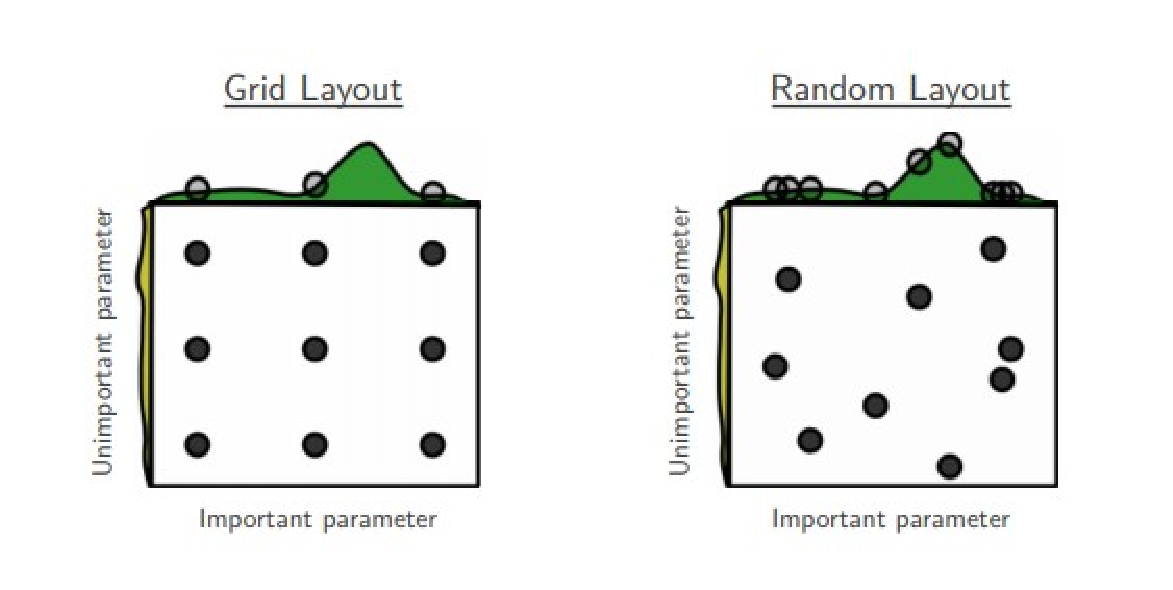
\includegraphics[scale=0.7]{images/chapter_2/random_search.eps}}
\caption{Grid and random search \citep[from][]{bergstra2012random}}
\label{fig:Grid and Random Search}
\end{figure}
In Figure \ref{fig:Grid and Random Search} the grid search and random search of nine trials are compared for optimising a generic function $f(x, y) = g(x) + h(x)$ where Above each square $g(x)$ is shown in green, and left of each square $h(y)$ is shown in yellow. With grid search, nine trials only test $g(x)$ in three distinct places. With random search, all nine trials explore distinct values of $g$. This failure of grid search is the rule rather than the exception in high dimensional hyper-parameter optimisation.

\subsubsection{Iterative methods} \label{Iterative methods}

\citet{bergstra2011algorithms} carried out a state of the art of hyper-parameter optimisation methods for deep neural network models. This work shows the interest of iterative optimisation, based on the criterion of the Expected Improvement of the model performance, proposed by \citep{jones2001taxonomy}. The study introduces two optimisation methods. One method seeks to model the optimisation problem by \textit{Gaussian stochastic processes} (GP) and the second TPE (\textit{Tree-structured Parzen Estimator}) method proposes a kernel-based modelling. These methods are based on the construction of meta-models. The study highlighted the superiority of these two methods over the optimisation by random sampling. 

In the context of this research work we applied solely the TPE algorithm. The Tree-structured Parzen Estimator (TPE) is a sequential model-based optimisation (\textit{SMBO}) approach. SMBO methods sequentially construct models to approximate the performance of hyper-parameters based on historical measurements, and then subsequently choose new hyper-parameters to test based on this model. The TPE approach models $P(x|y)$ and $P(y)$ where x represents hyper-parameters and y the associated quality score. $P(x|y)$ is modelled by transforming the generative process of hyper-parameters, replacing distributions of the configuration prior with non-parametric densities.

In this subsection we have shown how hyper-parameters can be optimised. Whether it is carried out through a random sampling approach or through the use of iterative methods, hyper-parameter optimisation is an expensive task in terms of computation time. The cost of optimising these models is very high, due to the infinity of possible architectures and the many hyper-parameters, especially for neural networks. In the following subsection, we will present an approach that allows to reduce the overall computational time and which facilitates the convergence of the model, especially if the number of samples composing the training set is not particularly high.


\subsubsection{Transfer learning} \label{Transfer Learning}

Transfer learning is biologically motivated by the way that humans apply learned knowledge to solve new problems, and consists in exploiting knowledge learned in one problem and searching a good protocol of transferring to a new problem.
In practice, in transfer learning problems, a parametric model is trained in the source problem and transferred to the target problem in a special way, like transferring parameters, or considering the relations between problems. This approach become particularly interesting when we deal with a dataset where the number of samples is small. There is no a well-defined rule to distinguish between a small and a large dataset. Moreover, the amount of data required to solve a machine learning problem depends on the task that we try to accomplish. In the context of this research project we consider as small, every dataset that have less than 1000 samples. 

Convolutional networks are broadly applicable in the fields mentioned before. The success of transfer learning with convolutional networks relies on the generality of the learned representations that have been constructed from a large database like ImageNet \citep{deng2009imagenet}. \citet{yosinski2014transferable} quantified the transferability of these pieces of information in different layers, e.g. the first layers learn general features, the middle layers learn high-level semantic features and the last layers learn the features that are very specific to a particular task. \citet{zeiler2014visualizing} also visualised the features in the intermediate layers, demonstrating, with images, that convolutional networks learn features from general level to task-specific level. Overall, the learned representations can be conveyed to related but different domains and parameters in the network are reusable for different tasks. The intuition behind transfer learning for image-related tasks is that if a model is trained on a large and general enough dataset, this model will effectively serve as a generic model of the visual world. You can then take advantage of these learned feature maps without having to start from scratch by training a large model on a large dataset.

In practice, we distinguish two successive stages in the training of a neural network by transfer learning: the training of the new last layers, and then the specialisation of the whole network. The first stage is to guarantee the convergence of the classifier on the new task. We seek to obtain a satisfactory inference score. This is why in a first step, only the weights of the neurons of the new last layers are adjusted by back-propagation of the error gradient. Once the convergence of the last layers has been obtained, it is possible to fine-tune the whole network by performing an adjustment of all the weights of the layers in order to improve the classification score.


\section{Conclusion}

In the manufacturing industry, product quality is an indicator for evaluating the production capacity of a company. Customers are increasingly demanding in terms of product quality and providing the customer with a product that complies with the specifications is absolutely essential in a market that is becoming more and more competitive. The best possible solution to deliver 100\% of compliant parts to the customer would be to inspect in details all parts produced. However, most companies cannot test every single product. There may simply be too high a volume or number of them to inspect at a reasonable cost or within a reasonable time frame. Or effective testing might result in the destruction of the product or render it unfit for sale in some way. Moreover, traditional process control approach does not take into account the relationship between process data and produced part quality. In this chapter we have described a general approach that can be applied every time that we want to take advantage of an historical set of data to improve manufactured parts quality. The presented data-driven approach requires four main stages: data acquisition, data processing, exploratory data analysis and machine learning modelling. Data acquisition involves the task of identifying all the input process data, as well as the output quality data, that are interesting to try to solve our quality improvement use-case. Data processing is the task of processing and filtering raw input data in order to reduce the noise within data and to make data suitable for machine learning modelling. Exploratory data analysis could be used for better understanding the correlation between data and to eventually fine tune the data processing stage. Finally, machine learning modelling allows to build a model which relate input process data and output quality data. In this way it is possible, for a new set of input data, to provide the prediction, or inference of the quality of the finished part. Moreover, using an interpretable model it is possible to identify which process parameters affect the most manufactured parts quality and eventually improve process monitoring. There exists a wide variety of machine learning algorithms. In the second section of this chapter we have presented the linear regression and the linear models with a penalisation term, Tree-Based methods, Support Vector Machines and a few Deep-learning architectures that we have applied throughout our research work. In the following chapters we will present an application of this method in the industrial context studied along this doctoral studies.


\subsection{Industrial contribution}

From the industrial point of view, this chapter describes a new way of monitoring processes and controlling quality. Instead of relying on acceptance sampling, the historical data can be used to infer a model able to provide real-time quality inspection without any direct measurement of the part. This leads to two major benefits:

\begin{itemize}
    \item Faster detection of quality non-conformities. By providing a quality status for each part produced, it is possible to quickly react and adjust the production process to prevent occurrence of new non-conformities.
    \item Reduced destructive testing. If the model is reliable enough to provide accurate results, it is possible to reduce the number of destructive tests that are regularly performed to assess part quality.
    \item Better understanding of the production process. If the machine learning model is interpretable, it is possible to identify which process parameters that most affect part quality. In this way, it is possible to fine-tune the process by focusing more attention to the control of important parameters. 
\end{itemize}

\cleardoublepage